\documentclass{article}
\usepackage{tikz, comment}
\usepackage{pifont}
\usepackage{fontspec}
\usetikzlibrary{arrows, decorations.markings, decorations.pathreplacing}
\begin{comment}
:Title: Not defined yet
:Tags: upper;revolution;positive;periodic;period;multiple;lower
:Author: Prof.Hu Ji-shan, HKUST
:Slug: No name yet

Description Here.........
\end{comment}
\begin{document}\centering

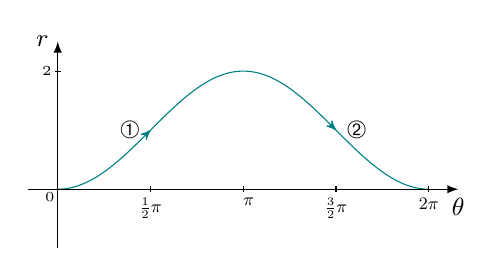
\begin{tikzpicture}[>=latex,xscale=.5*1.5, yscale=.5*1.5][font=\sf\small]

\draw[->, >=stealth', teal, samples=150, smooth, domain=0:pi/2, variable=\t]
plot ({\t}, {1-cos(\t r)}) -- ({pi/2}, {1-cos(pi/2 r)});
\draw[->, >=stealth', teal, samples=150, smooth, domain=pi/2:3*pi/2, variable=\t]
plot ({\t}, {1-cos(\t r)}) -- ({3*pi/2}, {1-cos(3*pi/2 r)});

\draw[teal, samples=150, smooth, domain=3*pi/2:2*pi, variable=\t]
plot ({\t}, {1-cos(\t r)});

%\draw[xstep=1cm,ystep=1cm,color=gray!80] (0, -1) grid (8, 8);
\foreach \x in {}
\draw (\x,2pt/6) -- (\x,-2pt/6)
node[anchor=north] {\tiny$\x$}
;
\draw ({pi/2},2pt/1.5) -- ({pi/2},-2pt/1.5)node[anchor=north, xshift=0, scale=0.7] {$\frac{1}{2}\pi$};
\draw ({pi},2pt/1.5) -- ({pi},-2pt/1.5)node[anchor=north, xshift=2, scale=0.7] {$\pi$};
\draw ({3*pi/2},2pt/1.5) -- ({3*pi/2},-2pt/1.5)node[anchor=north, xshift=0, scale=0.7] {$\frac{3}{2}\pi$};
\draw ({2*pi},2pt/1.5) -- ({2*pi},-2pt/1.5)node[anchor=north, xshift=0, scale=0.7] {$2\pi$};

\foreach \x in {}
\draw (\x,2pt/2.5) -- (\x,-2pt/2.5)
node[anchor=south] {\tiny$\x$}
;
\foreach \y in {2}
\draw (-2pt/1.5,\y) -- (2pt/1.5,\y)
node[anchor=east] {\tiny $\y$}
;

\draw[->] (-0.5, 0) -- ({2*pi+0.5}, 0)node[below] {\small $\theta$} ;
\draw[->] (0, -1) -- (0, 2.5)node[left] {\small $r$} ;

\node at ({pi/2-.35}, 1) {\ding{192}};
\node at ({3*pi/2+0.35}, 1) {\ding{193}};


\node at (-0.2/1.5, -0.2/1.5) {\tiny$0$};

\end{tikzpicture}\hskip0.5cm
\end{document}